\documentclass[a4paper]{article}

\usepackage[english]{babel}
\usepackage[utf8]{inputenc}
\usepackage{amsmath}
\usepackage{graphicx}
\usepackage{color}
\usepackage{subcaption}

\usepackage{algorithm}
\usepackage{algorithmicx}
\usepackage{algpseudocode}

\begin{document}

\title{Term Project Report: Estimation of Population Size Based on Diploid Whole Genome Seuqence}
\author{Mikhail Kolmogorov}
\maketitle

\section{Introduction}

The important question one could ask is whether it is possible to track the change of the size for
a given population during its history. While we usually observe only current state
of a population, it seems to be possible to make some conclusions about significant
changes in size that occur through the evolution (bottlenecks or exponentional grows). 
In their paper from 2009, Li and Durbin describe a method based on HMM simulation,
which is then used for estimation of the population sizes of different human populations.
The algorithm models discrete changes in size and requires only two copies of a chromosome as input.
The results are in agreement with the common knowledge about some important
events in the human history.

While Li and Durbin's approach marked an important advancement in the population estimation
problem the described algorithm seems to be hard to understand. Here we want to consider
a simplier model of population evolution and show that using simple techniques one
could apply this model to the same kind of data (a pair of chromosomes) and get an
approximation of hidden parameters.

\section{Results}

\subsection{Problem Overview}

The model we want to consider describes an evolution of a population, which has
a rapid change in size from $N_1$ to $N_2$ at time $t_c$, measuring from
the point of observation (see figurure~\ref{fig:model}). Assuming that we are given the size $N_1$ at
the beginning, two unknowns remain in the model: $r = N_2/N_1$ and $t_c$.

\begin{figure} [h]
\centering
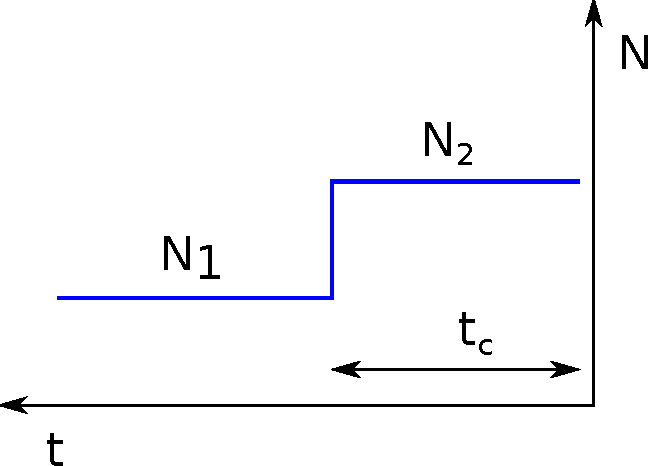
\includegraphics[width=0.5\textwidth]{model.pdf}
\caption{An overview of the model.}
\label{fig:model}
\end{figure}

Let us consider a pair of chromosomes, that are given as an input. Because of the 
rearrangement events happened during the evolution, these chromosomes are splitted
into smaller regions which are characterised by high LD values for loci pairs inside.
We will assume that those regions have independent evolution history. Thus,
instead of two chromosomes, we have many pairs of corresponding regions, which are
independent from each other. For each pair of regions we could measure the heterozygosity
rate (the number of differences between two sequences) which is correlated with the time
passed from the MRCA to these two regions. It gives us a set of values, that
represent a distribution of heterozygosity rate for a pair of chromosomes. As the time 
for two individuals to coalescence depends on the population size (namely, 
$P[\tau=t] = e^{\frac{-t}{N}}$ for a population of constant size), we expect to see
some variance in the heterozygosity distribution as the size of the population changes.

\subsection{Simulation}

We performed the simulation as follows. First, the genome is split into the regions of
size 1Mb, which corresponds to high-LD segments (without recombination inside). Each of
those regions is then modelled independently. For a given pair of regions we need to
model their coalescence time. To do this, we first assume that they have coalesced
after the time point $t_c$. Then, $P[t] = e^{\frac{-t}{N_2}}$ so we draw a 
value $t_2$ from exponential distribution with parameter equal to $\frac{1}{N_2}$. 
If $t_2 \leq t_c$, we keep that value and set the coalescense time to $t_2$. 
Now let us suppose, that the opposite is true.
Then, the coalescence has happened before the population size was changed and we
need to calculate $P[t | t_2 > t_c]$ which is simply $e^{\frac{-t}{N_1}}$, because
exponential distribution is memoryless. Thus, if for $t_2 > t_c$, we draw $t_1$
from exponential distribution with parameter $\frac{1}{N_1}$ and set the coalescence time
to $t_1 + t_c$. Then, number of mutations is calculated as $\tau \cdot \mu \cdot l$, 
where $\mu$ is
a per-site mutation rate ($1.1 * 10^{-8}$) and $l$ is a length of a region. This
procedure is repeated for every pair of regions. The heterozygosity
distribution could be estimated by a histogram. See the examples of such histograms for
different model parameters on figure~\ref{fig:hist}.

\begin{figure}[h!]
\centering
\begin{subfigure}[b]{0.49\textwidth}
	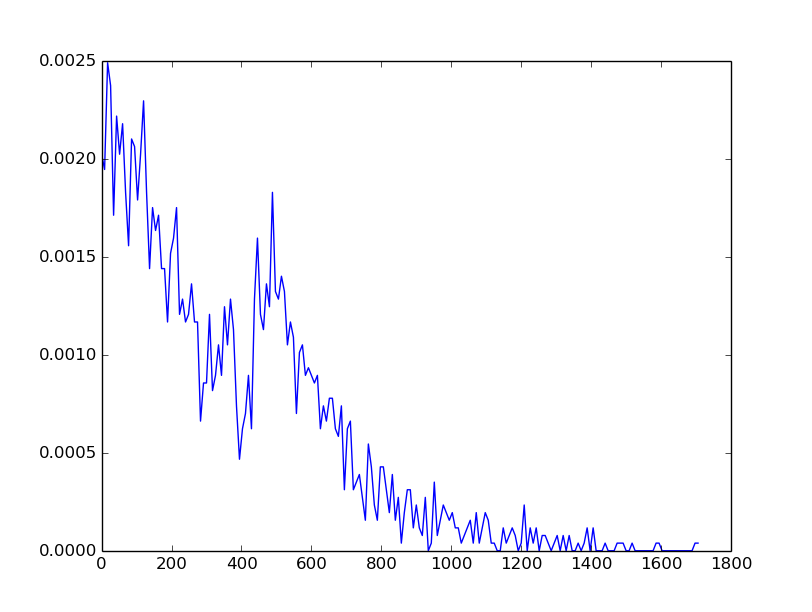
\includegraphics[width=\textwidth]{figure_2_20000.png}
	\caption{$r = 2$, $t_c = 20000$}
\end{subfigure}
\begin{subfigure}[b]{0.49\textwidth}
	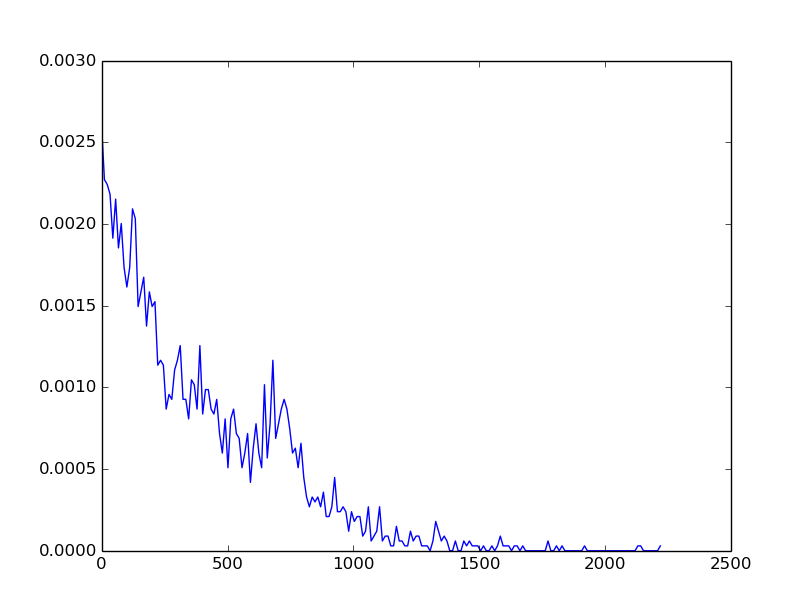
\includegraphics[width=\textwidth]{figure_2_30000.png}
	\caption{$r = 2$, $t_c = 30000$}
\end{subfigure}
\begin{subfigure}[b]{0.49\textwidth}
	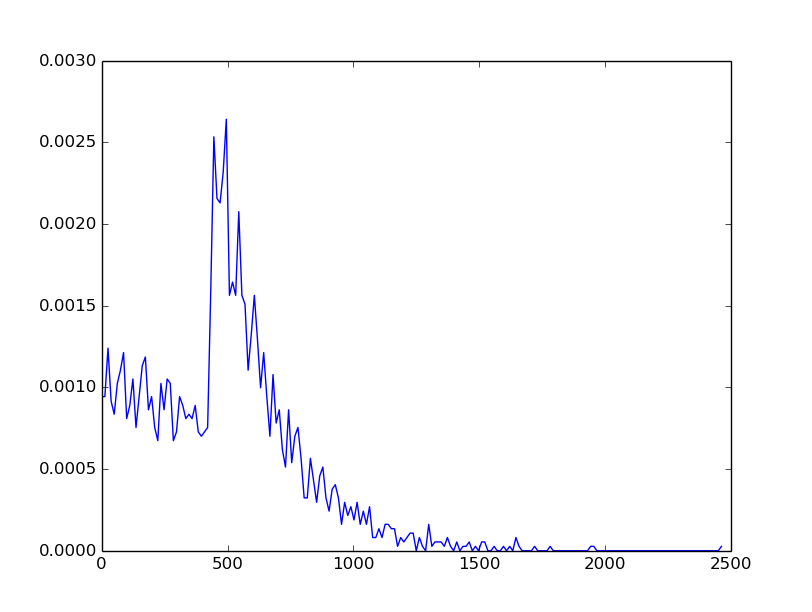
\includegraphics[width=\textwidth]{figure_4_20000.png}
	\caption{$r = 4$, $t_c = 20000$}
\end{subfigure}
\begin{subfigure}[b]{0.49\textwidth}
	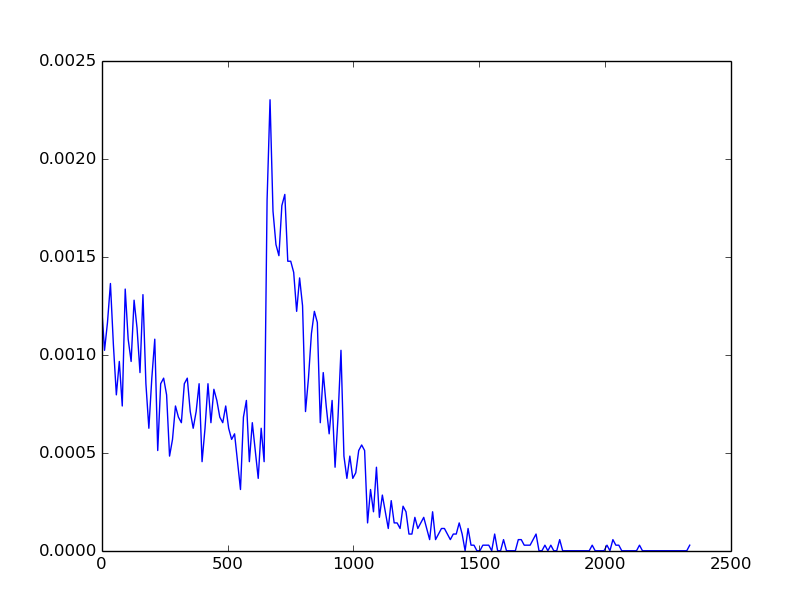
\includegraphics[width=\textwidth]{figure_4_30000.png}
	\caption{$r = 4$, $t_c = 30000$}
\end{subfigure}
\caption{Estimated heterozygosity distribution for different model parameters.}
\label{fig:hist}
\end{figure}

\subsection{Fitting Distribution Parameters}

Now, given a histogram, we want to estimate the hidden model parameters, $r$
and $t_c$. Based on the heterozygosity histogramms 
we want to assume that the heterozygosity density distribution has a form: 
\begin{equation}
\pi_1 \lambda_1 e ^ {\frac{-t}{\lambda_1} } + \pi_2 \lambda_2 e ^ {\frac{-(t + s)}{\lambda_2} }
\end{equation}

Thus, given a joint distribution of two exponentials, we need to separate them, inferring
hidden parameters $\pi$, $\lambda$ and $s$. Expectation-Maximization (EM) algorithm applies
very naturaly for this kind of problems. However, it is hard to include shift $s$ into the
model, because it could not be robustly estimated from the data (due to the nature of
exponential distribution, which is not continious from the left). Thus, we first estimate $s$
independently from the other parameters (as a highest peak in a histogram) and then
plug its value into EM. The algorithm converges relatively fast and an example of 
the estimation could be seen at the figure~\ref{fig:em}

\begin{figure} [h]
\centering
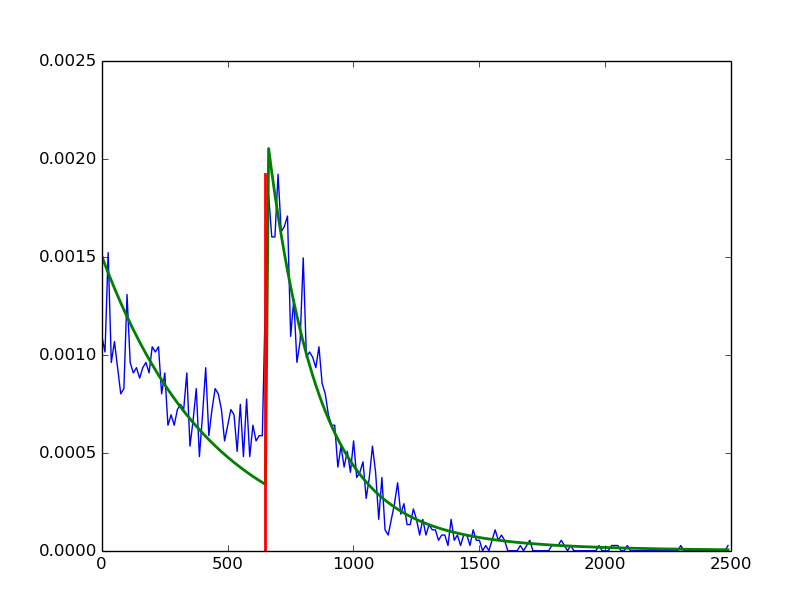
\includegraphics[width=0.7\textwidth]{figure_em.png}
\caption{Fitting distribution parameters with EM algorithm.}
\label{fig:em}
\end{figure}

\subsection{Inferring $r$ and $t_c$}

To study how the underlying model parameters $r$ and $t_c$ depend on distribution
parameters $\pi$ and $\lambda$, we performed a set of simulations with various
values of $r$ and $t_c$ and then performed a linear regression analysis. $t_c$
exibits a linear dependence on $s$ with a high $R^2$ value, suggesting that
$t_c$ is a linear function of $s$ and could be retrived directly from the estimate
of $s$. See the residuals vs fitted plot on figure~\ref{fig:lm_time}.

\begin{figure} [h]
\centering
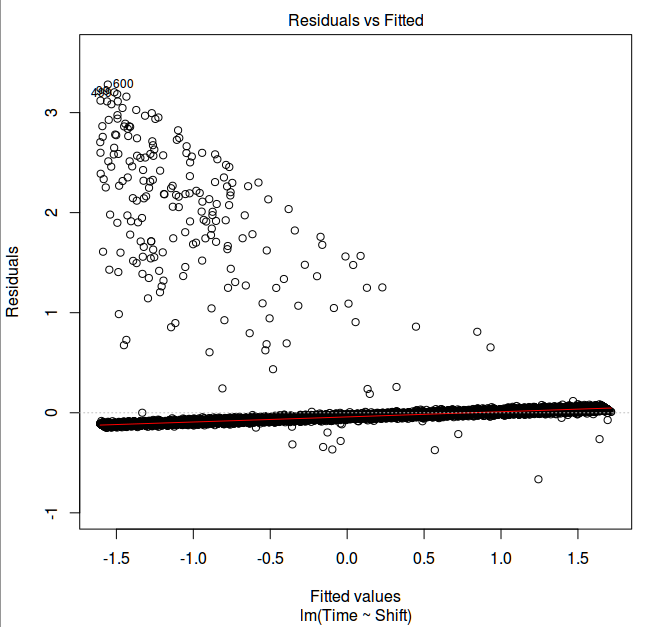
\includegraphics[width=0.7\textwidth]{figure_lm_time.png}
\caption{Linear regression of $t_c$ over $s$.}
\label{fig:lm_time}
\end{figure}

The other parameter, $r$ seems to be having more complicated form of dependance, rather than linear.
However, a term $e^{\frac{-t}{N_2}}$ seems to be in a linear dependence with $\pi_2$, which explains
about $85\%$ of variance. See the correponding plot on the figure~\ref{fig:lm_exp}. This part of the
study needs further investigations.

\begin{figure} [h]
\centering
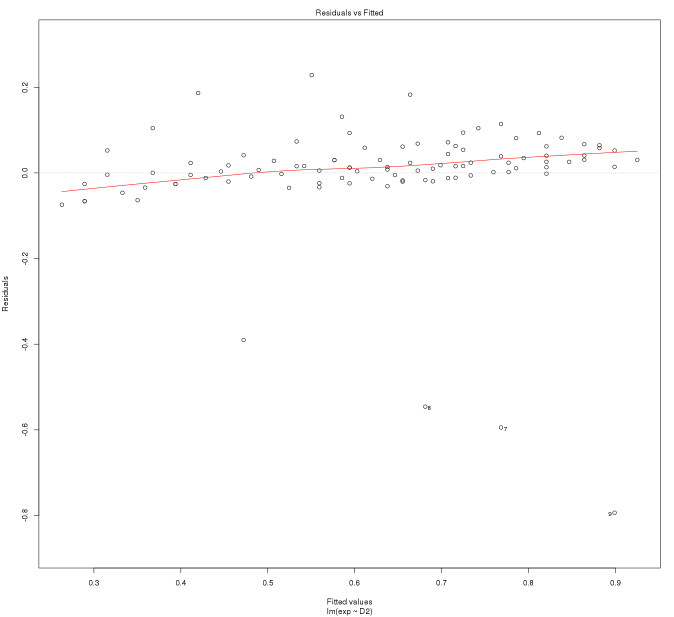
\includegraphics[width=0.7\textwidth]{figure_lm_exp.png}
\caption{Linear regression of $e^{\frac{-t}{N_2}}$ over $\pi_2$.}
\label{fig:lm_exp}
\end{figure}

\section{Discussion}

In this report we describe a simple model of population evolution, where it exibits
a rapid change in size at the given point of time. We performed simulations and showed
that it is possible to infer the hidden parameters of the model based on a data
from a pair of chromosomes.

However, some some aspects remain uninvestigated. First, the important question to ask
is if the performed simulations reflects the behaviour of a real population, which
follows out model. For instance, the non-recombinant chromosomal regions were chosen
to be equally long, however it is not true for a real genome. This aspect could bring
some additional noise to the observed signal, which will complicate the further analysis.

Second, the shift parameter $s$ should be estimated more rapidly. We have observed a fraction
of outliers in our linear model analysis, which might be associated with a wrong estimation of $s$.

Third, the final question remains unanswered: how to get the value of $r$ given the fitted values of
$\pi$, $\lambda$ and $s$.

\end{document}
